\documentclass{article}
\usepackage[utf8]{inputenc}
\usepackage{natbib}
\usepackage{graphicx}
\usepackage[]{endfloat}
\usepackage[dvipsnames]{xcolor}
\usepackage{longtable,pdflscape, graphicx, booktabs, dcolumn, listings, amsmath,bbm,courier,pgffor,fixltx2e, natbib,enumerate,amssymb,amsfonts,color,hyperref,array,calc,multirow,tikz,amsthm,anyfontsize,bbm}
\DeclareDelayedFloatFlavour*{longtable}{table}
\title{Public-private wage gap in Brazil: a counterfactual analysis using longitudinal data}
\author{Vítor Costa}
\date

\begin{document}

\maketitle
\tableofcontents

\section{Introduction and motivation}
Anecdotal evidence in Brazil suggests public sector workers are overcompensated compared to their private sector counterparts. In fact, (brief list of references for the Brazilian economy and their estimates). (Highlight the discrepancy of these estimates). (highlight their lack of treatment for endogenous selection).

Add
\begin{enumerate}
    \item Segmentation (the two different legal frameworks, CLT vs Statutory)
    \item Endogenous selection (selection via highly competitive civil exams)
    \item Increasing share of personnel expense in the national budget 
    \item Results for other countries
\end{enumerate}


This paper's contribution to this literature is twofold: I apply a quantile Oaxaca-Blinder decomposition method and use the panel structure of the data to estimate worker fixed effects. The method allows me to estimate composition and structural effects of the private-public gap along the distribution of wages. Endogeneity procedure relies on \cite{canay_simple_2011}.  

Add 
\begin{enumerate}
    \item conclusions
    \item sections layout 
\end{enumerate}

\section{Previous Evidence}\label{section:lit-review}

\section{Brazilian Civil Service Panorama}

\section{Data}
The data come from the \emph{Relatório Anual de Informações Sociais}, or simply, RAIS. The RAIS is a yearly based data set of matched employer-employee administrative records kept by the Brazilian federal government to primarily consolidate the information necessary for the execution of social programs, such as social security and benefits for low earners. It also aims to subsidize policy makers dependent on labor market statistics. \\

\noindent
The collection of data from  business establishments was implemented in 1975, by force of law, and since 1997 the collection is done electronically. RAIS covers the whole universe of the formal labor market in Brazil. As of 2007, it contained information from 6.9 million establishments and 37.6 workers, approximately. \\

\noindent
The variables available from RAIS are varied. Each worker and establishment have their own unique identifier. An employer-employee observation contains data on monthly average earnings, occupation, industry sector, municipality of the establishment, date of worker admission, data of worker separation cause of separation - retirement, death, just cause etc - and tenure of the worker in the current job. The researcher can also observe employees demographic variables, such as race, gender, age, schooling, nationality, and disability status. \\

\subsection{Sample selection}
\noindent
The years in the data go from 2003 up to 2014, amounting to approximately 781 million observations. Due to the computational impossibility of estimating the model in the whole data, I select a 1\% sample based on the worker unique identifier. Following the standard practice in the literature, I filter the sample for prime age workers only, i.e. age between 25 and 54. For workers with more than one job, I keep only the record of the highest paying appointment. I also drop rural workers and employees under temporary contracts. The final sample has approximately 3.95 million job-year observations and 683,821 workers. \\

\subsection{Definition of Public Employees}
\noindent
I consider to public employees all workers whose employers are a part of the federal administration, thus including judicial, legislative and executive powers. The choice for the federal sphere is mainly motivated by the policy relevance of this paper. The federal budget is subject to bigger scrutiny from the other republican powers, the public, and international organisms. Secondly, due to the higher transparency in the National Treasury bookkeeping, I am able to provide a more reliable estimate for the fiscal impact of the public-private wage gap.        

\subsection{RAIS}
\begin{enumerate}
    \item Filter RAIS for: prime age workers (25-54), keep only CNPJs - drop CEIs, drop blank PIS, select only federal administration employees, keep only clt and statutory.
    \item sample using 1\% or 10\% of whole data set.  
    \item validate CNPJ and PIS
    \item compute log hourly wages (hired wages over hired hours)
    \item select contract types (permanent vs temporary)
    \item create variable for low, medium and high skills
    \item create different subsets from sample, skills $\times$ sex $\times$ race.
    \item show descriptive statistics.
\end{enumerate}

\subsection{Comparison with data in previous papers}
\begin{enumerate}
    \item describe advantages over PNAD
    \item describe advantages over PME
\end{enumerate}

\subsection{RAIS versus PNAD and PME}
The totality of papers mentioned in the literature review of Section \ref{section:lit-review} uses two different sources of employment records. The most widely used is the \emph{Pesquisa Nacional por Amostra de Domicílios} - or simply, PNAD - which is a household survey carried out yearly.  

\section{Equations for estimations}
\subsection{Naïve equations}
Throughout this paper I will refer to the model and estimation of the premium in the absence of any endogenous selection treatment as naïve. If we ignore the possibility of sorting into the public sector of individuals with higher unobserved ability, we could consistently estimate the public-private premium by means of an Oaxaca-Blinder decomposition[\cite{oaxaca_male-female_1973},\cite{blinder_wage_1973}]. \\

\noindent
Let's denote by $y^{1}_{it}$ the observed wage for individual $i$ in year $t$ in the public sector. If n year $t$, individual $i$ works at the private sector, I denote his wage by $y^{0}_{it}$. Conditional on a set $X_{it}$ of observed individual characteristics, the expected wage in each sector is given by  

\begin{align}
    y_{it}^{1} = X_{it}^{1}\beta^{1}+u_{it}\\
    y_{it}^{0} = X_{it}^{0}\beta^{0}+u_{it} \label{wage-priv}
\end{align}
which, after taking the averages over individuals, can be rewritten as
\begin{align}
    \bar{y}_{t}^{1} - \bar{y}_{t}^{0} &= \bar{X}_{t}^{1}\beta^{1} -\bar{X}_{t}^{0}\beta^{0} \\
    &= \underbrace{\left(\bar{X}_{t}^{1}-\bar{X}_{t}^{0}\right)\beta^{0}}_{Characteristics} +\underbrace{\bar{X}_{t}^{1}\left(\beta^{1}-\beta^{0}\right)}_{Structural} \label{ob-str}
\end{align}      

\noindent
The left hand side of equation (\ref{ob-str}) is the observed mean wage difference between public and private sector workers. The right hand side breaks this difference into two terms that I will refer to \emph{characteristics} and \emph{structural} effects. The characteristics estimates the size of the observed mean wage difference due to differences in observed attributes of workers in both groups, holding fixed the coefficients in the wage equation for group $0$. A higher characteristics effect is obtained when, holding fixed the parameters of equation (\ref{wage-priv}), workers in the public sector have higher (lower) mean observed attributes associated with positive (negative) coefficients in equation (\ref{wage-priv}). \\

\noindent
This is indeed the case when we observe the values of exploratory statistics from the sample. From table \ref{table:all}, we can see that workers in the public sector have higher education attainment, higher tenure in the current job, are slightly older and are more likely to be white.   

\begin{longtable}[c]{@{}lccc@{}}
\toprule
& Public (N=797128) & Private (N=3151791) & Total
(N=3948919)\tabularnewline
\midrule
\endhead
Hourly wage (2011 US\$) & & &\tabularnewline
- Mean (SD) & 41.314 (56.723) & 23.292 (56.803) & 26.930
(57.245)\tabularnewline
- Median (Q1, Q3) & 24.400 (12.444, 47.831) & 12.764 (9.224, 21.542) &
13.809 (9.548, 26.196)\tabularnewline
- Range & 1.141 - 4758.900 & 1.076 - 21991.700 & 1.076 -
21991.700\tabularnewline
Age & & &\tabularnewline
- Mean (SD) & 40.072 (8.129) & 35.858 (7.991) & 36.708
(8.196)\tabularnewline
- Median (Q1, Q3) & 40.000 (33.000, 47.000) & 34.000 (29.000, 42.000) &
36.000 (30.000, 43.000)\tabularnewline
- Range & 25.000 - 54.000 & 25.000 - 54.000 & 25.000 -
54.000\tabularnewline
Tenure & & &\tabularnewline
- Mean (SD) & 123.947 (102.908) & 41.529 (55.963) & 58.166
(75.708)\tabularnewline
- Median (Q1, Q3) & 95.300 (32.900, 200.900) & 20.900 (7.800, 50.900) &
26.800 (9.500, 72.900)\tabularnewline
- Range & 0.000 - 487.000 & 0.000 - 486.900 & 0.000 -
487.000\tabularnewline
Gender & & &\tabularnewline
- Male & 321731 (40.4\%) & 1973298 (62.6\%) & 2295029
(58.1\%)\tabularnewline
- Female & 475397 (59.6\%) & 1178493 (37.4\%) & 1653890
(41.9\%)\tabularnewline
Race & & &\tabularnewline
- N-Miss & 207504 & 16583 & 224087\tabularnewline
- White & 375817 (63.7\%) & 1981624 (63.2\%) & 2357441
(63.3\%)\tabularnewline
- Nonwhite & 213807 (36.3\%) & 1153584 (36.8\%) & 1367391
(36.7\%)\tabularnewline
Education & & &\tabularnewline
- Low & 194169 (24.4\%) & 1386563 (44.0\%) & 1580732
(40.0\%)\tabularnewline
- Medium & 315961 (39.6\%) & 1410160 (44.7\%) & 1726121
(43.7\%)\tabularnewline
- High & 286998 (36.0\%) & 355068 (11.3\%) & 642066
(16.3\%)\tabularnewline
\bottomrule
\label{table:all}
\end{longtable}

\begin{enumerate}
    \item Describe the Oaxaca-Blinder decomposition and outline the equation
    \item Describe the Quantile OB, methodology \cite{chernozhukov_inference_2013} 
\end{enumerate}
\subsection{Accounting for endogenous selection}
\begin{enumerate}
    \item Discuss \cite{canay_simple_2011} and outline equation for worker efffects estimation
    \item Outline net of FEs equation 
\end{enumerate}

\section{Estimation Results}
\subsection{Worker Effects}
The estimated distribution of worker effects is depicted in Figure \ref{fig:we}. The set of possible values for \textcolor{red}{$\alpha_i$ in equation XX is similar across both sectors}. It is not actually the range of individual effects that changes between the two sectors but the probability density of these effects. One can find public and private workers with practically any value for unobserved coefficients in that range, but it is notorious how the density of above average values is higher among public sector workers.\\

\begin{figure}[h!]\label{fig:we}
  \caption{Worker Effects by Sector}
  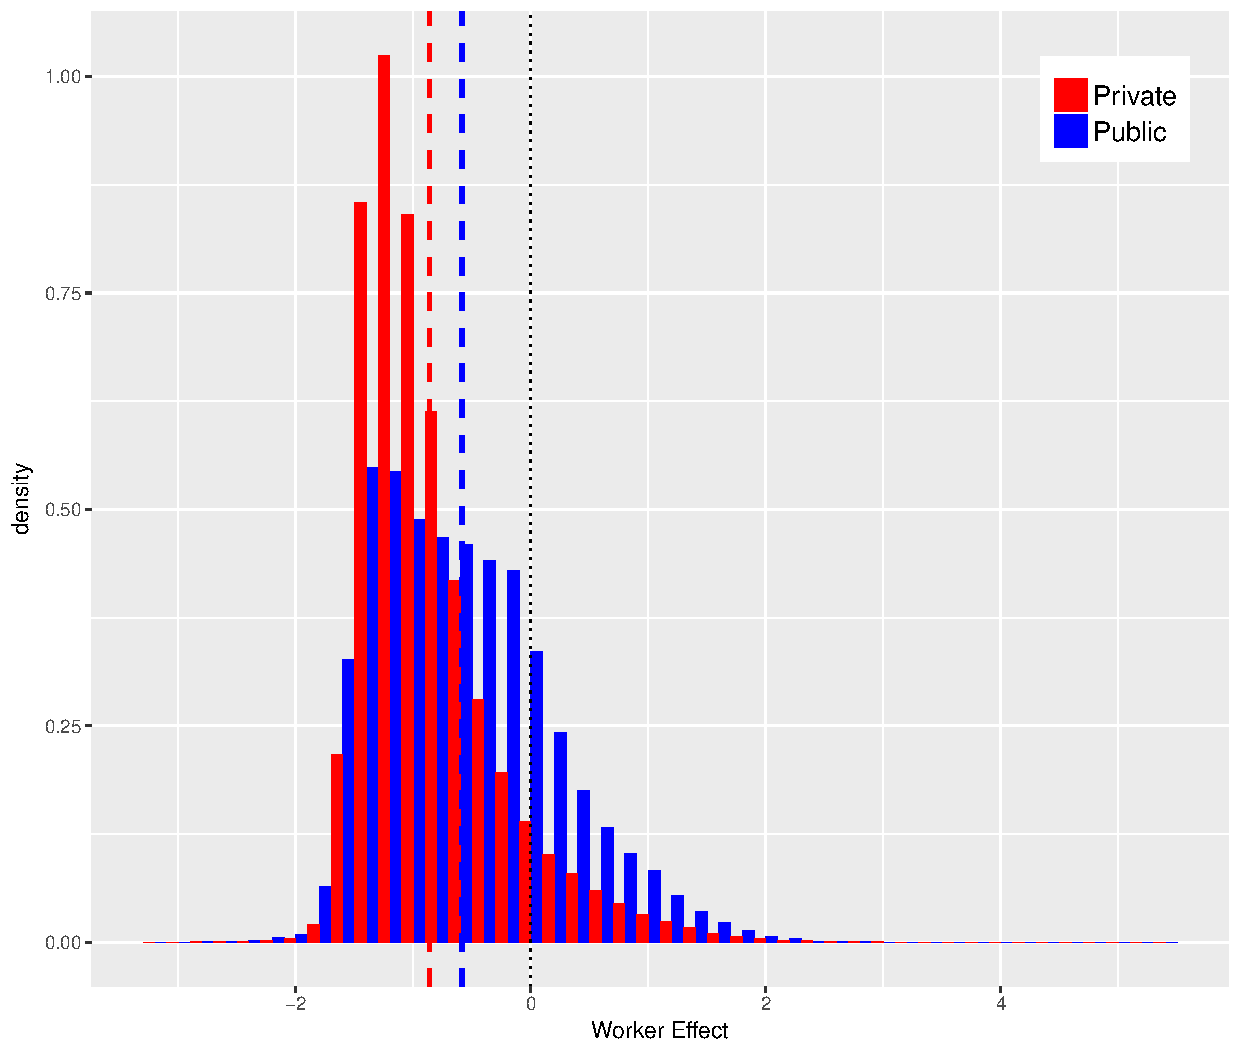
\includegraphics[scale=0.7]{graphs/001_fe_sector_onepc.pdf}
\end{figure}
\subsection{Oaxaca-Blinder (OB)}
\begin{enumerate}
    \item Report overall OB 
    \item Plot yearly OB in both cases
\end{enumerate}
The observed wage gap on the whole sample is of x\%, of which y\% is due to workers observed attributes differentials and the remainder z\% stems from differences in coefficients. From Figure \ref{fig:yearly}, the Oaxaca-Blinder decomposition shows that for the first four years in the sample the coefficients effect was negative for public employees, meaning that holding fixed their observed characteristics, their wages would be higher, on average, in the private sector. \\

\noindent
However, once we take the endogenous selection into the equation, not only does the overall premium get compressed but...


\begin{figure}[h!]
    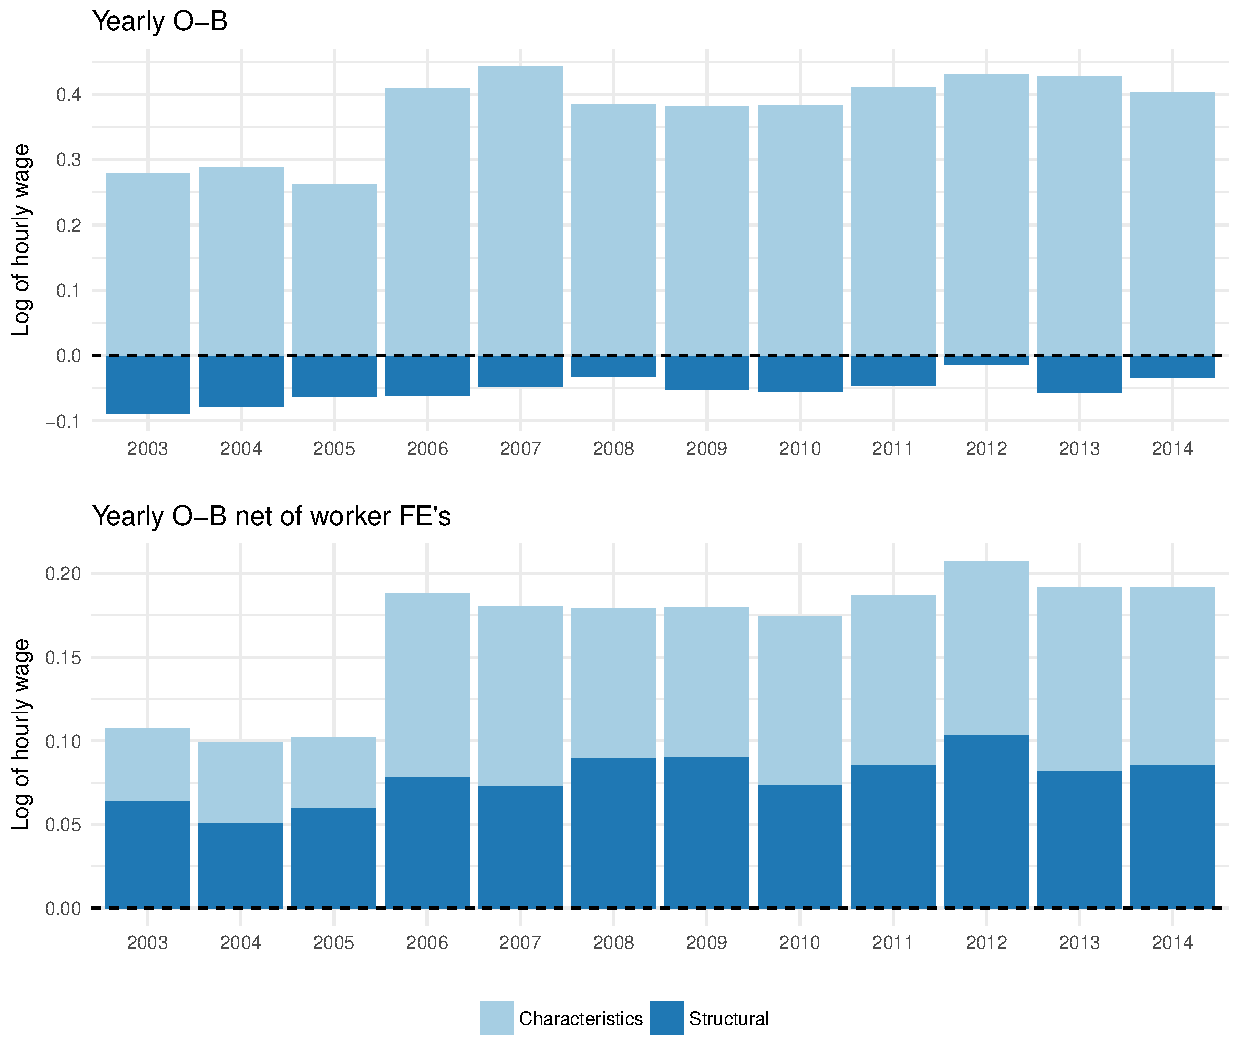
\includegraphics[scale=0.65]{graphs/002_yearly_ob_onepc.pdf}
    \caption{Oaxaca-Blinder Decomposition by Year}
    \label{fig:yearly}
\end{figure}
\subsection{Distribution of the Premium}
\begin{enumerate}
    \item Plot overall distribution in two cases
    \item Show distribution estimates broken by demographic groups
\end{enumerate}

\section{Conclusion}
 \begin{enumerate}
     \item what do we learn from the quantile decomposition? where does the premium phase out?
     \item is self-selection important? by how much?
     \item what is the size of premium once we account for selection?
     \item show expenses with inactive civil employees and its evolution in time.
     \item state the discrepancy of retirement entitlements for both types of workers and problems for future research. 
\end{enumerate}  

\newpage
\scriptsize{\bibliographystyle{chicago}}
\bibliography{library} %bibtex file name without .bib

\end{document}
